\documentclass[landscape,10pt]{article}
\usepackage[latin1]{inputenc}

\usepackage{ae}
\usepackage{amssymb}
\usepackage{url}
\usepackage{xspace}

\usepackage{tikz}
\usetikzlibrary{mindmap,trees}
\usetikzlibrary{shapes}

% set up externalization
\usetikzlibrary{external}
\tikzset{external/system call={latex \tikzexternalcheckshellescape -halt-on-error
-interaction=batchmode -jobname "\image" "\texsource";
dvips -o "\image".ps "\image".dvi;
ps2eps "\image.ps"}}
\tikzexternalize

%% https://www.bu.edu/math/files/2013/08/tikzpgfmanual.pdf

\begin{document}

\tikzstyle{root concept}+=[concept color=red!60]
%% \tikzstyle{level 1 concept}+=[set style={{every child}=[concept color=orange!50]}]
%% \tikzstyle{level 2 concept}+=[set style={{every child}=[concept color=blue!20]}]




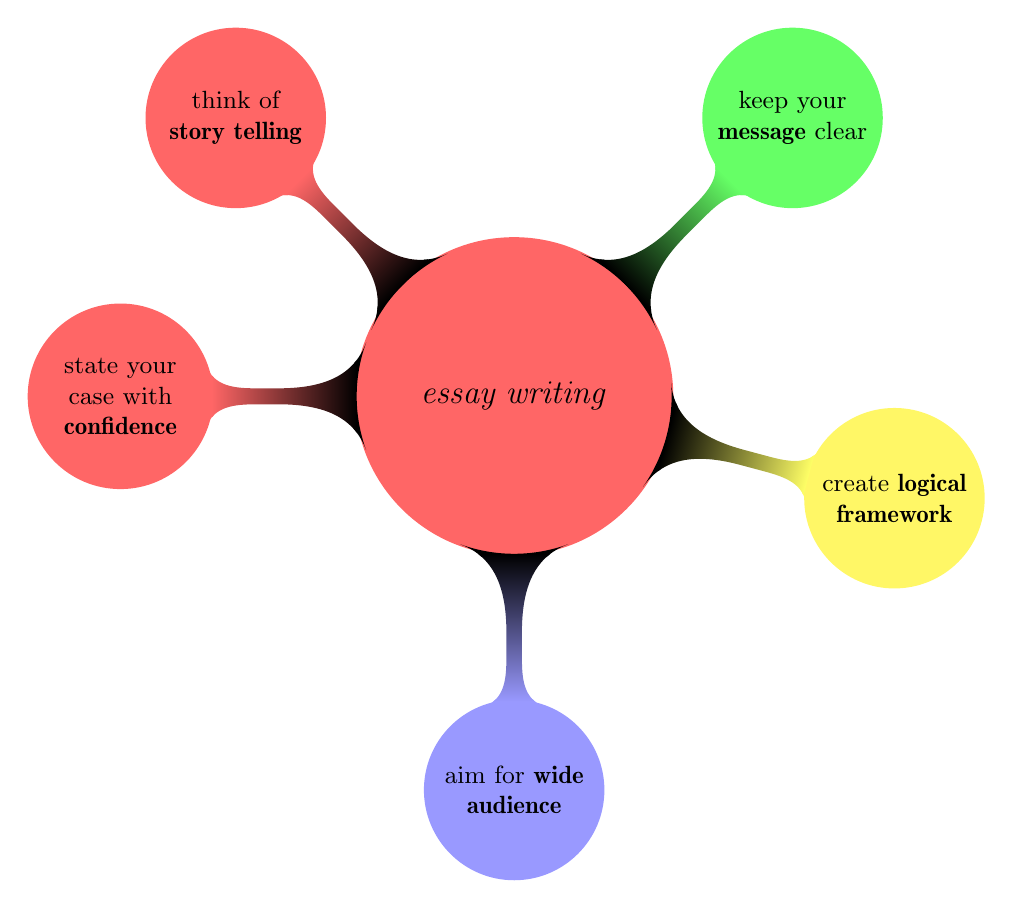
\begin{tikzpicture}[mindmap, level distance=30mm]
%%% 12-mark question %%%

      \node[concept, concept color=red!60] { \emph{essay writing}  }
      %% 
      child[grow=45, concept color=green!60]
      {
        node[concept, concept color=green!60] {keep your \textbf{message} clear} 
      }
      %% 
      child[grow=-15, concept color=yellow!60]
      {
        node[concept, concept color=yellow!60] {create \textbf{logical framework}} 
      }
       %% 
      child[grow=-180, concept color=red!60]
      {
        node[concept, concept color=red!60] {state your case with \textbf{confidence}} 
      }     
      %% 
      child[grow=135, concept color=red!60]
      {
        node[concept, concept color=red!60] {think of \textbf{story telling}} 
      }      
      child[grow=-90, concept color=blue!40] 
      {
        node[concept, concept color=blue!40] {aim for \textbf{wide audience} }
      }      
      ;


\end{tikzpicture}


\end{document}
